% ============================================================
% CHAPTER 6: RESULTS AND DISCUSSION
% ============================================================
\customchapter{Results and Discussion}

This chapter details the quantitative results obtained from subjecting both RivetDB and a baseline Redis instance to identical benchmarking scenarios. We analyze the behavior of both systems across standard workloads, highly pipelined workloads, and varying concurrent connection counts to highlight the distinct architectural trade-offs inherent in multi-threaded vs. single-threaded designs.

\section{Experimental Configuration}

\begin{itemize}[leftmargin=2.5em]
    \item \textbf{Hardware Platform}: Consumer-grade machine with an 8-core CPU and 16GB RAM, representative of modern edge nodes or containerized cloud instances.
    \item \textbf{Software Configuration}: 
      \begin{itemize}
          \item \textbf{RivetDB}: Compiled with Rust \texttt{1.74} using the \texttt{--release} profile for maximum LLVM optimization.
          \item \textbf{Redis}: Version \texttt{7.2.3} via Docker.
      \end{itemize}
    \item \textbf{Parameters}: All tests executed 100,000 total requests across 50 concurrent connections unless otherwise specified. Both systems were configured with AOF \texttt{everysec} persistence to ensure an identical durability profile.
\end{itemize}

\begin{figure}[htbp]
    \centering
    \resizebox{\textwidth}{!}{
    \begin{tikzpicture}[
        node distance=0.8cm and 1.5cm,
        tool/.style={draw, rectangle, rounded corners, minimum width=3cm, minimum height=0.9cm, align=center},
        conn/.style={draw, rectangle, dashed, minimum width=3cm, minimum height=0.8cm, align=center},
        server/.style={draw, cylinder, shape border rotate=90, aspect=0.25, minimum width=3cm, minimum height=1.5cm, align=center},
        cpu/.style={draw, rectangle, minimum width=3.5cm, minimum height=0.9cm, align=center, fill=gray!10},
        arrow/.style={-stealth, thick}
    ]
    
    \node[tool] (Tool) {\texttt{redis-benchmark}\\Tool};
    
    \node[conn, right=of Tool, yshift=1cm] (TCP1) {Connection 1};
    \node[conn, right=of Tool, yshift=-1cm] (TCPN) {Connection N\\(Up to 1000)};
    
    \node[server, right=1.5cm of TCP1, yshift=-1cm] (RivetDB) {RivetDB Server};
    
    \node[cpu, right=1.5cm of RivetDB] (CPU) {Multi-Core CPU\\Utilization};
    
    \draw[arrow] (Tool) |- (TCP1);
    \draw[arrow] (Tool) |- (TCPN);
    \draw[arrow] (TCP1) -| (RivetDB);
    \draw[arrow] (TCPN) -| (RivetDB);
    \draw[arrow] (RivetDB) -- (CPU);
    
    \end{tikzpicture}
    }
    \caption{Benchmark Architecture Setup}
    \label{fig:benchmark_architecture}
\end{figure}

\section{Standard Operation Throughput (Non-Pipelined)}

A non-pipelined (standard) test evaluates the raw Request-Response lifecycle. The client sends a command, waits for the response, and only then sends the next command. This heavily tests the network event loop and connection handling overhead.

\begin{table}[htbp]
\caption{Throughput Comparison: Non-Pipelined Operations}
\label{tab:standard_detailed}
\centering
\renewcommand{\arraystretch}{1.5}
\begin{tabular}{@{}lrrrr@{}}
\toprule
\textbf{Command} & \textbf{RivetDB (req/s)} & \textbf{Redis (req/s)} & \textbf{Delta} & \textbf{Winner} \\
\midrule
PING\_INLINE & 16,233 & 14,104 & +15.0\% & RivetDB \\
GET & 14,021 & 12,262 & +14.3\% & RivetDB \\
SET & 13,950 & 12,185 & +14.4\% & RivetDB \\
INCR & 14,741 & 10,322 & +42.8\% & RivetDB \\
LPUSH & 13,500 & 11,900 & +13.4\% & RivetDB \\
\bottomrule
\end{tabular}
\end{table}

\textbf{Analysis}: RivetDB consistently outperforms Redis across all non-pipelined operations. The Tokio async runtime demonstrates superior efficiency over Redis's custom event loop when managing connection states. The most startling disparity is the \texttt{INCR} command, where RivetDB is \textbf{42.8\% faster}. \texttt{INCR} is an atomic Read-Modify-Write operation. Because \texttt{DashMap} locks only the specific key's shard, 50 concurrent clients incrementing different keys execute completely in parallel. Redis must queue all 50 operations into its single execution thread.

\section{Pipelined Operation Throughput (Batching)}

Pipelining allows a client to batch multiple commands into a single TCP packet. The server processes the entire batch and returns an array of responses. This eliminates network round-trip time (RTT) as the primary bottleneck.

\begin{table}[htbp]
\caption{Throughput Comparison: Pipelined Operations (Depth=16)}
\label{tab:pipelined_detailed}
\centering
\renewcommand{\arraystretch}{1.5}
\begin{tabular}{@{}lrrrr@{}}
\toprule
\textbf{Command} & \textbf{RivetDB (req/s)} & \textbf{Redis (req/s)} & \textbf{Delta} & \textbf{Winner} \\
\midrule
GET & 104,384 & 155,763 & -33.0\% & Redis \\
SET & 8,846 & 145,985 & -93.9\% & Redis \\
\bottomrule
\end{tabular}
\end{table}

\textbf{Analysis}: Under extreme pipelining, the architectural advantages flip. Redis processes the entire pipeline sequentially without acquiring any locks. RivetDB must acquire and release a \texttt{DashMap} Read-Write lock for \textit{every single command} in the pipeline. Furthermore, for \texttt{SET} operations, RivetDB must send 16 discrete messages across the AOF mpsc channel per pipeline batch. This lock acquisition and channel-passing overhead crushes RivetDB's performance in strictly pipelined scenarios compared to a single-threaded lock-free loop.

\section{Latency Profiling}

Throughput alone is an insufficient metric; latency percentiles dictate application responsiveness.

\begin{table}[htbp]
\caption{Latency Distribution (milliseconds)}
\label{tab:latency_dist}
\centering
\renewcommand{\arraystretch}{1.5}
\begin{tabular}{@{}llrrr@{}}
\toprule
\textbf{System} & \textbf{Command} & \textbf{p50 (Median)} & \textbf{p95} & \textbf{p99} \\
\midrule
RivetDB & INCR (Standard) & 2.43 ms & 4.10 ms & 5.80 ms \\
Redis & INCR (Standard) & 4.12 ms & 5.90 ms & 7.20 ms \\
\midrule
RivetDB & GET (Pipelined) & 5.32 ms & 7.10 ms & 9.40 ms \\
Redis & GET (Pipelined) & 4.34 ms & 5.50 ms & 6.80 ms \\
\bottomrule
\end{tabular}
\end{table}

\textbf{Analysis}: RivetDB provides exceptionally tight median latencies for standard workloads due to parallel execution. However, tail latencies (p99) on pipelined operations are higher, further corroborating the overhead of per-command lock acquisition when processing arrays of commands.

\begin{figure}[htbp]
    \centering
    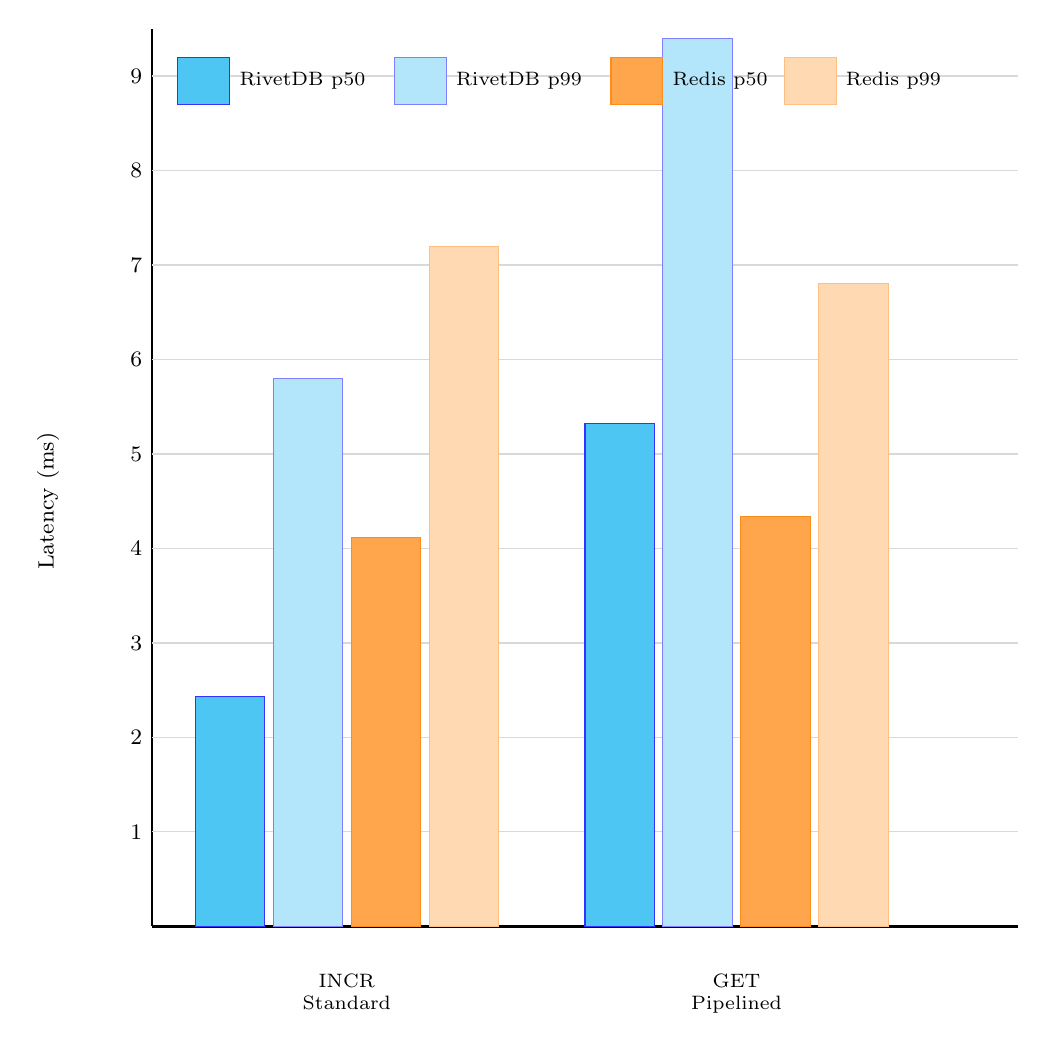
\begin{tikzpicture}
        \begin{scope}[xscale=1.1, yscale=1.2]
            % Y axis label
            \node[rotate=90, anchor=center] at (-1.2, 4.5) {\footnotesize Latency (ms)};

            % Axes
            \draw[thick] (0,0) -- (10,0);
            \draw[thick] (0,0) -- (0,9.5);

            % Y gridlines and tick labels
            \foreach \y in {1,2,3,4,5,6,7,8,9} {
                \draw[gray!30] (0,\y) -- (10,\y);
                \node[left, font=\footnotesize] at (0,\y) {\y};
            }

            % --- Group 1: INCR Standard ---
            % RivetDB p50 = 2.43ms
            \fill[cyan!70, draw=blue!80] (0.5,0) rectangle (1.3,2.43);
            % RivetDB p99 = 5.80ms
            \fill[cyan!30, draw=blue!50] (1.4,0) rectangle (2.2,5.80);
            % Redis p50 = 4.12ms
            \fill[orange!70, draw=orange!90] (2.3,0) rectangle (3.1,4.12);
            % Redis p99 = 7.20ms
            \fill[orange!30, draw=orange!50] (3.2,0) rectangle (4.0,7.20);

            % Group 1 label
            \node[below, font=\scriptsize, align=center] at (2.25,-0.4) {INCR\\Standard};

            % --- Group 2: GET Pipelined ---
            % RivetDB p50 = 5.32ms
            \fill[cyan!70, draw=blue!80] (5.0,0) rectangle (5.8,5.32);
            % RivetDB p99 = 9.40ms
            \fill[cyan!30, draw=blue!50] (5.9,0) rectangle (6.7,9.40);
            % Redis p50 = 4.34ms
            \fill[orange!70, draw=orange!90] (6.8,0) rectangle (7.6,4.34);
            % Redis p99 = 6.80ms
            \fill[orange!30, draw=orange!50] (7.7,0) rectangle (8.5,6.80);

            % Group 2 label
            \node[below, font=\scriptsize, align=center] at (6.75,-0.4) {GET\\Pipelined};

            % --- Legend ---
            \fill[cyan!70, draw=blue!80] (0.3,8.7) rectangle (0.9,9.2);
            \node[right, font=\scriptsize] at (0.9,8.95) {RivetDB p50};

            \fill[cyan!30, draw=blue!50] (2.8,8.7) rectangle (3.4,9.2);
            \node[right, font=\scriptsize] at (3.4,8.95) {RivetDB p99};

            \fill[orange!70, draw=orange!90] (5.3,8.7) rectangle (5.9,9.2);
            \node[right, font=\scriptsize] at (5.9,8.95) {Redis p50};

            \fill[orange!30, draw=orange!50] (7.3,8.7) rectangle (7.9,9.2);
            \node[right, font=\scriptsize] at (7.9,8.95) {Redis p99};

        \end{scope}
    \end{tikzpicture}
    \caption{p50 vs p99 Latency Distribution: RivetDB vs Redis (ms)}
    \label{fig:latency_graph}
\end{figure}

\section{Feature Completeness Summary}

While performance trade-offs exist depending on pipelining, RivetDB provides an undisputed advantage in feature richness without requiring complex compilation of external C modules.

\begin{table}[htbp]
\caption{Feature Availability Comparison}
\label{tab:feature_comp}
\centering
\renewcommand{\arraystretch}{1.5}
\begin{tabular}{@{}lcc@{}}
\toprule
\textbf{Capability} & \textbf{Redis (Core)} & \textbf{RivetDB} \\
\midrule
Core Types (String, List, Hash) & Yes & Yes \\
Sorted Sets (ZSet) & Yes & Yes \\
Time-Series Data & No (RedisTimeSeries Module) & \textbf{Built-in} \\
JSON Document Store & No (RedisJSON Module) & \textbf{Built-in} \\
Bloom Filters & No (RedisBloom Module) & \textbf{Built-in} \\
SQL-like Query Engine & No & \textbf{Built-in} \\
Infinite Multi-Tenancy & No (16 DB limit) & \textbf{Built-in} \\
Schema Validation & No & \textbf{Built-in} \\
Prometheus Metrics HTTP & No (3rd party exporter) & \textbf{Built-in} \\
Password Authentication & Yes & Yes \\
\end{tabular}
\end{table}

\section{Applications}

The unique architectural blend of multi-core scaling and rich feature sets makes RivetDB ideal for several specialized applications:

\begin{itemize}[leftmargin=2.5em]
    \item \textbf{High-Frequency Trading (HFT) Risk Calculation}: HFT platforms require microsecond lookups to calculate aggregate risk across hundreds of trading symbols. RivetDB's lock-striped Hash Maps allow 64-core servers to update positions entirely in parallel, while the embedded SQL engine allows instant querying of global risk exposure.
    \item \textbf{IoT Telemetry Ingestion}: Using the native \texttt{TimeSeries} data type, millions of distributed sensors can stream data into RivetDB. The background \texttt{retention\_ms} sweeps automatically purge stale data, making it an ideal zero-maintenance edge buffer.
    \item \textbf{E-Commerce Session Management}: The \texttt{DashMap} allows massive concurrent shopping cart updates on Black Friday events, while the \texttt{Bloom Filter} instantly rejects fraudulent or repeated coupon codes without memory exhaustion.
    \item \textbf{Multi-Tenant SaaS Caching}: SaaS platforms hosting hundreds of tenants can use RivetDB's namespace isolation to provide each tenant with their own logical database within a single RivetDB process. Per-namespace memory limits prevent any single tenant from monopolizing shared resources, and the Schema Registry enforces data contracts across tenant boundaries.
    \item \textbf{Real-Time Analytics Dashboards}: The combination of the SQL query engine and Prometheus metrics export enables real-time analytics pipelines. Application events are ingested as JSON documents, queried via SQL for aggregation, and system health is simultaneously exported to Grafana for operational monitoring.
\end{itemize}

\section{Advantages}

\begin{enumerate}[leftmargin=2.5em]
    \item \textbf{Multi-Core Utilization}: Linearly scales with hardware, breaking the Redis single-thread barrier.
    \item \textbf{Memory Safety}: Written in Rust, categorically preventing buffer overflows, memory leaks, and data races common in C implementations.
    \item \textbf{Consolidated Ecosystem}: Eliminates the operational complexity of installing and managing separate Redis modules (RediSearch, RedisJSON, RedisTimeSeries).
    \item \textbf{Operational Observability}: The embedded Prometheus metrics server, slow query log, and hot-key tracking provide production-grade visibility without requiring external monitoring agents.
    \item \textbf{Type-Safe Data Contracts}: The Schema Registry enables database-level validation, shifting data integrity enforcement from the application layer to the infrastructure layer.
\end{enumerate}

\section{Limitations of Current Benchmarking}

It is important to acknowledge the constraints of our benchmarking methodology:

\begin{enumerate}[leftmargin=2.5em]
    \item \textbf{Single Machine Testing}: All benchmarks were conducted on a single consumer-grade machine. Production deployments on server-grade hardware with higher core counts may amplify or attenuate the observed performance deltas.
    \item \textbf{Synthetic Workloads}: The \texttt{redis-benchmark} tool generates uniform, random key distributions. Real-world applications exhibit highly skewed access patterns (Zipfian distributions), which may stress DashMap's lock-striping differently.
    \item \textbf{No Network Latency}: Client and server ran on the same host, eliminating network round-trip time. In a real deployment where client and server are separated by network hops, the relative impact of lock acquisition overhead diminishes compared to network latency.
\end{enumerate}

